\documentclass[a4paper, 12pt]{article}
\usepackage[utf8]{inputenc}
\usepackage[lmargin=3cm, tmargin=3cm, rmargin=2cm, bmargin=2cm]{geometry}
\usepackage[onehalfspacing]{setspace}
\usepackage[T1]{fontenc}
\usepackage[brazil]{babel}

%%%\usepackage{amssymb, amsmath, mathptmx}%bigominus

\usepackage{wasysym}%male and female

\usepackage{graphicx, graphics, xcolor, comment, enumerate, multirow, multicol, indentfirst}

\usepackage{amsmath, amsthm, amsfonts, amssymb, dsfont, mathtools}
\everymath{\displaystyle} 

\usepackage{blindtext}

\usepackage[round]{natbib}
\bibliographystyle{apalike}

\usepackage{hyperref}

%Code packages:
\usepackage{listings}
\usepackage{xcolor}

%New colors defined below
\definecolor{codegreen}{rgb}{0,0.6,0}
\definecolor{codegray}{rgb}{0.5,0.5,0.5}
\definecolor{codepurple}{rgb}{0.58,0,0.82}
\definecolor{backcolour}{rgb}{0.95,0.95,0.92}

%Code listing style named "mystyle"
\lstdefinestyle{mystyle}{
  backgroundcolor=\color{backcolour},   commentstyle=\color{codegreen},
  keywordstyle=\color{magenta},
  numberstyle=\tiny\color{codegray},
  stringstyle=\color{codepurple},
  basicstyle=\ttfamily\footnotesize,
  breakatwhitespace=false,         
  breaklines=true,                 
  captionpos=b,                    
  keepspaces=true,                 
  numbers=left,                    
  numbersep=5pt,                  
  showspaces=false,                
  showstringspaces=false,
  showtabs=false,                  
  tabsize=2
}

%"mystyle" code listing set
\lstset{style=mystyle}

\title{Projeto 4: Tomografia Computadorizada}
\author{
  Herberth Luan Vieira Oliveira\\
  \texttt{12559110}
  \and
  Juliana de Abreu Faria\\
  \texttt{10336275}
  \and
  Victor Viana de Oliveira Matos\\
  \texttt{11810821}
  \and
  Vinícius da Costa Collaço\\
  \texttt{11811012}
  \and
  Vitor Sillos Alonso\\
  \texttt{9506935}
}

\begin{document}

\maketitle

\section{Introdução}
    O trabalho tem como objetivo de apresentar as aplicações e a construção do modelo matemático apresentado na década de 70 pelo programador britânico Goldfrey Hounsfield que trabalhou junto com um profissional da neurorradiologia. Com trabalho deles foi possível as imagens internas do cérebro humano.
    
\subsection{Resumo do Artigo}
O processo para retirada de imagens internas da parte do corpo humano foram batizadas por teus criadores (Goldfrey) como tomografia computadorizada axial transversa.

A técnica desenvolvida parte de uma reconstrução de imagens bidimensionais com seções transversais  junto a fluxos de raios X unidimensionais que vão passando pelo corpo do paciente.
A construção da imagem se dará pelos raio X que passam no corpo e são captados pelos detectores e são convertidos em energia elétrica, e logo um estímulo elétrico para o computador formar a imagem.

\subsubsection{As construções das equações lineares}

Para que o computador monte as imagens o algoritmo montando precisa resolver uma série de equações lineares, como trata-se de diversas equações é mencionado que no artigo é utilizada o artifício da Técnica de Reconstrução Algébrica (TRA), que, normalmente, utiliza-se para achar os valores aproximados de sistemas lineares como se formarão e suas soluções serão a base para formação da imagem da tomografia.

O escaneamento de um corpo no artigo estudado é dado de duas formas : modo paralelo e modo leque, o estudado nesse trabalho é o primeiro, ou seja, modo paralelo.

\begin{center}
    \caption{Modo paralelo:'Escaneamento' por meio de Raio X}
    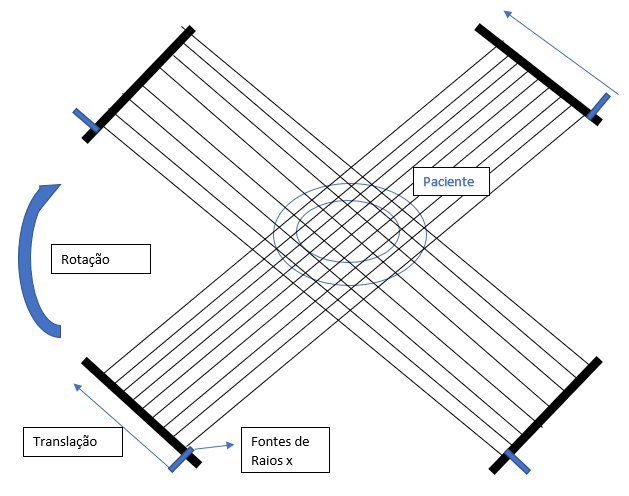
\includegraphics[width=11cm]{Figura1.png}
    \source{Fonte: Feito pelo próprio autor.}
\end{center}


Como é próprio do nome, modo paralelo, os raios X passaram pelo corpo de maneira paralela e unidimensional, mas os raios que são detectados são aqueles que não ultrapassam (absorvida) o corpo ou desviados, fazendo um par fonte-detector é girado de um pequeno ângulo e é feito um novo conjunto de medidas; o processo se repete até chegar o número de medidas que se almeja, abaixo está a imagem do que foi descrito.

\begin{center}
    \caption{Um dos feixes de Raio X ultrapassando o corpo}
    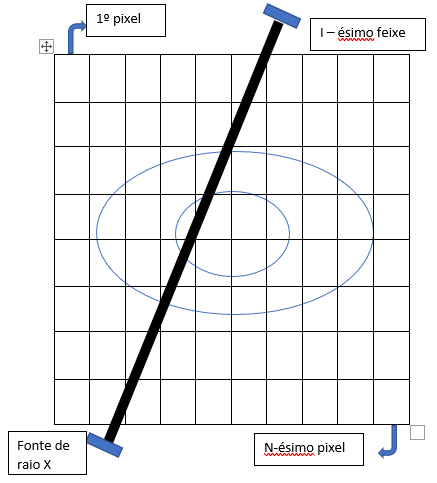
\includegraphics[width=8cm]{Figura2.png}
    \source{Fonte: Feito pelo próprio autor.}
\end{center}

Essa imagem apresenta a secção transversal e imagem construída no feixes de raios X, como se percebe ela é dividida em pixels que vão e 1 a N. Para construção da imagem imagina-se que o paciente está sendo "bombardeado" por raios X e também se tem a ideia de cada pixel será "igualmente bombardeado" pelo feixes de Raios X.

Portanto, o objetivo é determinar a densidade de Raios X em cada pixel. A diferenciação da densidade é dada uma tonalidade de cinza, isso se dá pelo fato da diferença de absorção dos feixes de raios X em diferentes tecidos do corpo humano.

A densidade de raios X absorvida pelo j-ésimo pixel é dado por $x_j$ e é definida:

   $$x_{j}= ln\left(\frac{\mathrm{número\ de\ fótons\ entrando\ no\ j-esimo\ pixel}}{\begin{matrix}
\mathrm{número\ de\ fótons\ saindo\ do\ j-ésimo\ pixel}
\end{matrix}}\right)$$

Aplicando a propriedade logarítmica ln(a/b) = -ln(b/a), temos:

    $x_j$ = -ln(fraçao de fótons que passa pelo j-ésimo pixel sem ser absorvida)
    
E para um dado feixe, temos que a seção de fótons que passa por uma fileira de pixeis deve ser igual à fração de protons que passa pela seção tranversal sem ser absorvida.


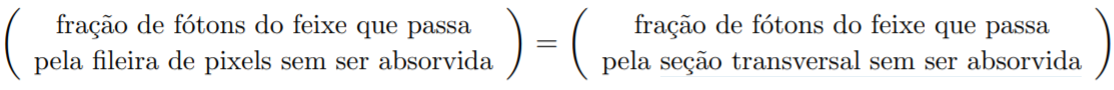
\includegraphics[width=11cm]{figura fluxo.png}


Dessa maneira, dada uma densidade b obtida empiricamente com calibrações do aparelho de tomografia e variáveis x1, x2...xn sendo as diversas densidades desconhecidas, obtemos a seguinte equação:
    
    $$x_1+x_2+...+x_n=b1$$
    
Ademais, de maneira análoga aos casos horizontais ou verticais, se considerarmos os feixes que passam por cada pixel de linhas ou colunas que constem em $$j_1, j_2,..., j_n$$, então temos que:
$$x_j1 + x_j2 + ... + x_jn$$
Se definirmos o coeficiente a como sendo:

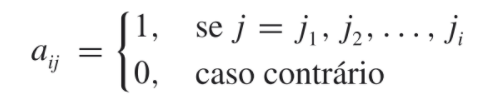
\includegraphics[width=9cm]{coef a.png}

Podemos reescrever a equação acima como:

$$a_{i1}*x_1 + a_{i2}*x_2 + ... + a_{in}*x_n = b_n$$

Isto posto, se considerarmos um escaneamento completo com M equações, teremos o sistema abaixo:
$$a_{11}*x_1 + a_{12}*x_2 + ... + a_{1n}*x_n = b_1$$
$$a_{21}*x_1 + a_{22}*x_2 + ... + a_{2n}*x_n = b_2$$
$$a_{31}*x_1 + a_{32}*x_2 + ... + a_{3n}*x_n = b_3$$
$$a_{M1}*x_1 + a_{M2}*x_2 + ... + a_{Mn}*x_n = b_M$$
    
Este sistema de equações com M equações e N variáveis, para este projeto, será considerado com M > N, na qual existem mais feixes do que pixels no campo de visão. Devido a erros experimentais e de modelagem, dificilmente encontraremos uma solução exata para o sistema de equações. Para tanto, podemos nos utilizar de algorítimos para encontrar soluções aproximadas.

Para este exemplo, utilizaremos um algoritmo pertencente à classe de Técnicas de Reconstrução Algébrica (TRA). Neste algoritmo, dado um número de equações que não possuem intersecção em comum, não existe uma única solução exata. Porém, a área formada pela intersecção de conjuntos de equações estão situados relativamente próximos e podem ser considerados como uma solução aproximada do sistema.

Para obter essa solução aproximada, são usados os seguintes passos:



\begin{center}
    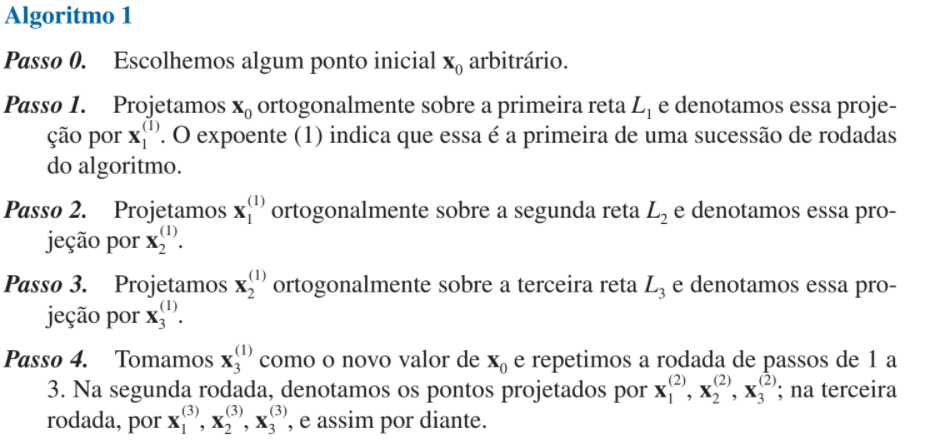
\includegraphics[width=11cm]{algoritimo.png}
    \source{Fonte: Lell et al., 2015}
\end{center}

Este algorítimo gerará sequências de pontos, na qual um valor x1* se aproximará da reta L1, um valor x2* se aproximará da reta L2 e assim por diante, de maneira que as iterações do algorítimo não irão além destes pontos, sendo portanto conhecido como o ciclo limite.

Para o cálculo da projeção ortogonal, usamos a seguinte equação:


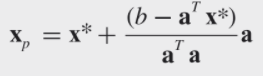
\includegraphics{projeção ortogonal.png}



Para testar o algorítimo, serão consideradas três equações:


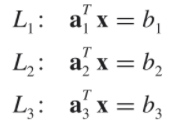
\includegraphics{equacoes.png}

    
Na qual temos os valores:


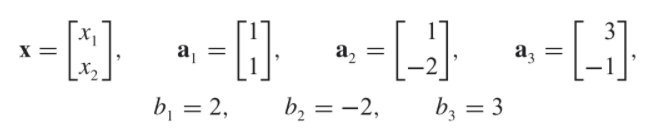
\includegraphics{coeficientes.png}


Ao rodar o algorítimo 6 vezes, é possível ver os resultados na imagem a seguir:


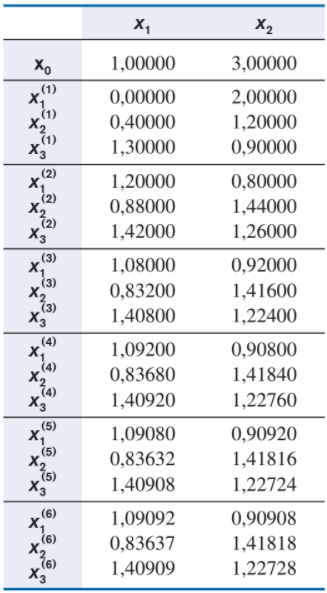
\includegraphics{resultados.png}
    
Os resultados obtidos ao final das rodadas estão visíveis na figura a seguir

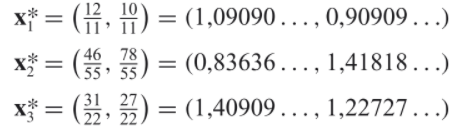
\includegraphics{x estrela.png}

    
\subsection {Atualidade}   
O algorítimo CAT de tomografia auxiliada por computadores (do inglês computerized axial tomography) foi implementado com sucesso por Godfrey N. Hounsfield para realização de exames em larga escala. O exame se utiliza da tirada de diversas imagens ao redor de um eixo axial para conseguir obter as relações de densidade dos materiais e assim gerar as imagens.

O primeiro paciente examinado com esta tecnologia ocorreu no hospital de Atkinson Morley em Londres \citep{lell2015evolution}, sendo este fato um marco uma nova era no estudo clínico. Originalmente, o exame usava uma técnica rotacional sobre um eixo, na qual eram obtidas imagens a cada 1 grau rotacionado. Ao todo o exame levava em torno de 5 minutos.

Nas chamadas tecnologias de primeira e segunda geração \citep{lell2015evolution}
os scans eram feitos apenas na região da cabeça. Com a chegada da terceira geração, foram introduzidas imagens obtidas com rotação de 360 graus. Em 1987, com a introdução de tecnologia de sistema em rotação contínua os tempos de ciclo de 1s. Procedimentos CT feito em fluxos espirais foram introduzidos em 1989 e trouxeram uma nova perspectiva em imagens 3D para tomografias. Em 2005, com a introdução de DSCT (Dual Source Computorized Tomography) houve um grande avanço na definição das imagens e tempos de processamentos. Com este avanço, iniciou-se uma corrida por um aumento de definição das imagens.

Para típicas imagens médicas, o eixo X-Y simboliza o eixo transversal do paciente, enquanto que o eixo Z simboliza o eixo longitudinal. Um típico vetor consiste de 800 a 1000 detectores no eixo transversal, com até 320 detectores no eixo Z \citep{lell2015evolution}. A vantagem de um maior número de detectores no eixo Z é um maior número de detalhes no eixo longitudinal. Em 1992, a empresa Elscint introduziu no mercado o primeiro equipamento CT com 2 detectores. Dessa maneira, em 1998 outras empresas concorrentes introduziram no mercado equipamentos com 4 detectores. Com isso teve início uma corrida por detectores, culminando no equipamento Toshiba Aquilion One, com 320 Detectores \citep{lell2015evolution}. Alguns modelos de inovação com suas principais características podem ser vistos na figura a seguir, mostra-se as características dos equipamentos:
\begin{center}
    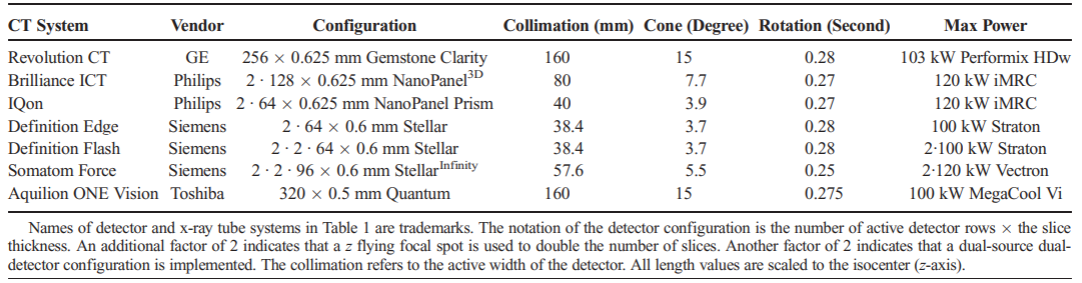
\includegraphics[width=16cm]{modelos ct.png}
    \source{Fonte: Lell et al., 2015}
\end{center}
        
\section{Algoritmos}

\subsection {Bibliotecas Utilizadas}

Nesse trabalho foi utilizada a linguagem Python com a utilização das seguintes bibliotecas:

\begin{lstlisting}[language=Python, caption=Import de bibliotecas, label=listing_bibliotecas] 
import numpy as np
import pandas as pd
from skimage import io
from skimage import data
import matplotlib.pyplot as plt
import math
\end{lstlisting}

No decorrer do relatório e transcrição dos códigos serão as bibliotecas serão utilizadas com os codinomes adotados no código acima.

\subsection{Projeção Ortogonal}

\begin{lstlisting}[language=Python, caption=Projeção Ortogonal, label=listing_ProjecaoOrtogonal] 
def ProjecaoOrtogonal (a,b,x_star):
  #Funcao para achar o ponto ortogonal entre a reta ax = b e o ponto x*
  num = b - (np.dot(a.T,x_star))
  den = np.dot(a.T,a)

  xp = x_star + num/den*a

  return xp
\end{lstlisting}

O algoritimo para achar a projeção ortogonal de um ponto em relação à uma reta (pensando em um plano cartesiano), foi baseado na equação descrita no início. O algorítimo foi criado para funcionar com qualquer tamanho de vetor, e retorna um vetor coluna.

\begin{center}
    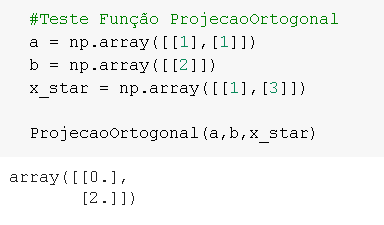
\includegraphics[width=8cm]{08_Teste_Projecao_Ortogonal.PNG}
    
    Teste Função Projeção Ortogonal.
\end{center}

\subsection{Algoritimo 1}

\begin{lstlisting}[language=Python, caption=Algoritimo1, label=listing_Algoritimo1] 
def Algoritmo1 (a1,a2,a3,b1,b2,b3,x,n):
  resultado = []
  resultado.append(np.array(x))
  x0 = ProjecaoOrtogonal(a1,b1,x)

  for i in range (n):
    x1 = ProjecaoOrtogonal(a1,b1,x0)
    resultado.append(x1)
    x2 = ProjecaoOrtogonal(a2,b2,x1)
    resultado.append(x2)
    x3 = ProjecaoOrtogonal(a3,b3,x2)
    resultado.append(x3)
    x0 = x3
  
  return resultado
\end{lstlisting}

O Algorítimo1 usa o algorítimo de Projeção Ortogonal, para o caso de resolução de um sistema linear com 3 linhas, se pensarmos em um plano, ou 3 equações lineares. No exemplo abaixo a resolução do exemplo mostrado no livro com o algorítimo construído.

\begin{center}
    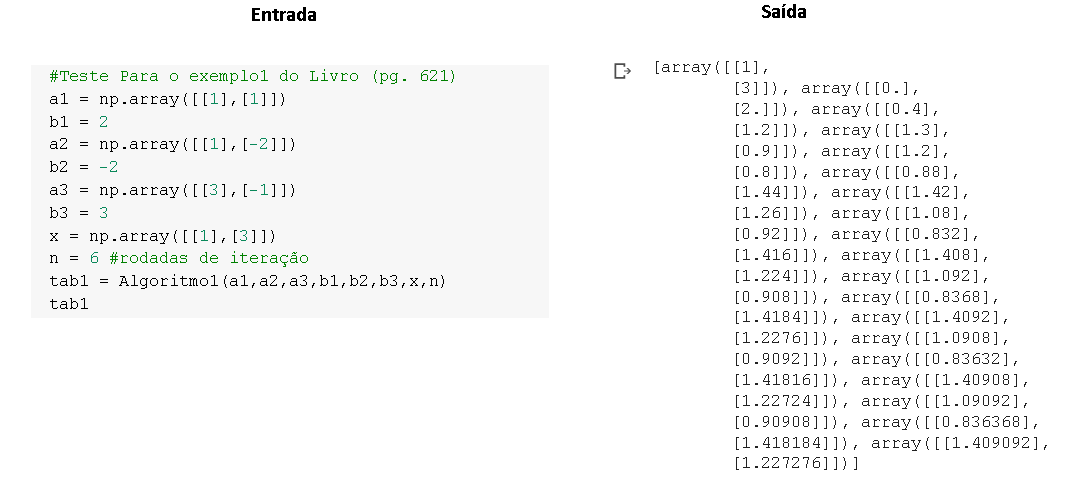
\includegraphics[width=16cm]{09_Teste_Algoritimo1.PNG}
    
    Teste do Algorítimo1.
\end{center}
 
Para cada iteração no Algorítimo1, valor 'n', tem a saída de 3 vetores colunas de duas dimensões, que graficamente representam os 3 pontos resultantes do sistema, na 6 iteração já tem uma boa convergência.

Para melhor apresentação, o resultado foi transformado em um DataFrame.

\begin{lstlisting}[language=Python, caption=Tabela 1 em DataFrame, label=listing_Tab1toDF] 
Tabela1 = pd.DataFrame()

#Df apartir de tab1 (resultado do ex1)
for i in range (len(tab1)):
  Tabela1 = Tabela1.append(tab1[i].T.tolist())

#Renomeando Colunas e resetando o index
Tabela1.rename({0:'X1',1:'X2'},inplace=True,axis=1)
Tabela1 = Tabela1.reset_index().drop('index',axis=1)
Tabela1
\end{lstlisting}

\begin{center}
    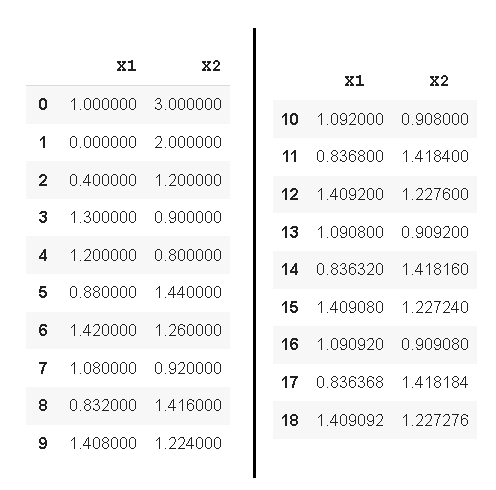
\includegraphics[width=8cm]{10_Exemplo1_DF.PNG}
    
    Teste do Algorítimo1.
\end{center}

O algorítimo converge bem rapidamente, na sexta interação temos o valor convergindo na quarta casa decimal. Na imagem do resultado podemos ver a conversão comparando os últimos 2 grupos de resultados (linhas 13, 14 e 15 comparado com as linhas 16, 17 e 18)

\subsection{Algoritimo2}

\begin{lstlisting}[language=Python, caption=Algorítimo2, label=Algoritimo2]
def Algoritmo2 (a,b,xstar,n):
  
  resultado = []
  lenb = len(b)
  resultado.append(np.atleast_2d(xstar)) #primeiro resultado
  xstarC = np.atleast_2d(xstar).T #lista em vetor coluna
  x0 = ProjecaoOrtogonal(np.array(a[0].T),b[0],xstarC)

  for j in range(n):
    for i in range (lenb):
      x0 = ProjecaoOrtogonal(np.array(a[i].T),b[i],x0)
      resultado.append(x0.T)
   
  
  return resultado
\end{lstlisting}

O Algorítimo 2, generaliza o primeiro algorítimo para um cenário além de equações no plano, para um hiperplano. Na entrada o algorítimo recebe a matriz a, onde cada linha representa um mapeamento das equações, a lista b, com os resultados das equações, o ponto inicial (xstar) e o número de iterações 'n'. Como resultado final é produzido uma lista de arrays.

\subsubsection{Teste Algoritimo2}

\begin{lstlisting}[language=Python, caption=entradas, label=Algoritimo2_entradas]
#Matriz vetor a
a =np.matrix([[0,0,0,0,0,0,1,1,1],
              [0,0,0,1,1,1,0,0,0],
              [1,1,1,0,0,0,0,0,0],
              [0,0,0,0,0,1,0,1,1],
              [0,0,1,0,1,0,1,0,0],
              [1,1,0,1,0,0,0,0,0],
              [0,0,1,0,0,1,0,0,1],
              [0,1,0,0,1,0,0,1,0],
              [1,0,0,1,0,0,1,0,0],
              [0,1,1,0,0,1,0,0,0],
              [1,0,0,0,1,0,0,0,1],
              [0,0,0,1,0,0,1,1,0]])
#Valores de b
b = [13.0, 15.0, 8.0, 14.79, 14.31, 3.81, 18.0, 12.0, 6.0, 10.51, 16.13, 7.04]
xstar = np.zeros(9)
\end{lstlisting}

como exemplo para teste do algorítimo, usamos o problema prático de uma imagem de 9 pixels. A primeira equação no exemplo é:

$$x_7+x_8+x_9=13.0$$

e como vetor inicial, começamos em um vetor zerado.

\begin{lstlisting}[language=Python, caption=Calculo e Saída, label=Algoritimo2_saida]
tab2 = Algoritmo2(a,b,xstar,45)

Tabela2 = pd.DataFrame()

#Df apartir de tab2
for i in range (len(tab2)):
  Tabela2 = Tabela2.append(tab2[i].tolist())

#Renomeando Colunas e resetando o index
Tabela2.rename({0:'x1', 1:'x2', 2:'x3', 
                3:'x4', 4:'x5', 5:'x6',
                6:'x7', 7:'x8', 8:'x9'}, inplace=True,axis=1)
Tabela2 = Tabela2.reset_index().drop('index',axis=1)
Tabela2.round
\end{lstlisting}

\begin{center}
    \includegraphics[width=12cm]{11_Saida_Algorítimo2.PNG}
    
    Teste do Algorítimo2.
\end{center}

O algorítimo como foi construído inicialmente tem um problema que consome muita memória RAM sem necessidade, pois ele guarda todos os valores das iterações, mas só precisamos do último valor, pois é o valor convergido. No exemplo a última linha corresponde o resultado do algorítimo para os 9 pixels.

\subsection{Algoritimo Generalizado}

\begin{lstlisting}[language=Python, caption=Algorítimo Generalizado, label=AlgoritimoGeneralizado]
def Algoritmo2 (a,b,xstar,n):
  
  lenb = len(b)
  xstarC = np.atleast_2d(xstar).T #lista em vetor coluna
  x0 = ProjecaoOrtogonal(np.array(a[0].T),b[0],xstarC)

  for j in range(n):
    for i in range (lenb):
      x0 = ProjecaoOrtogonal(np.array(a[i].T),b[i],x0)
   
  
  return x0.T
\end{lstlisting}

Para a otimização de uso de memória o Algorítimo2 foi feita uma pequena alteração para só retornar a última linha, sendo assim possível usar o modelo em construção de imagens maiores.


\section{Problema Prático $3\times 3$}

A \textbf{i-ésima equação de feixe} tem o seguinte formato para $N$ pixels:

$$a_{i1}x_1+a_{i2}x_2+...\ +a_{iN}x_N=b_i$$

Calcularemos as 12 equações do tipo definido acima para cada um dos três métodos (do centro do pixel, da reta central e da área).

Considerando as especificações dos feixes dadas, temos que os 4 conjuntos de feixes são da seguinte forma:

\begin{center}
    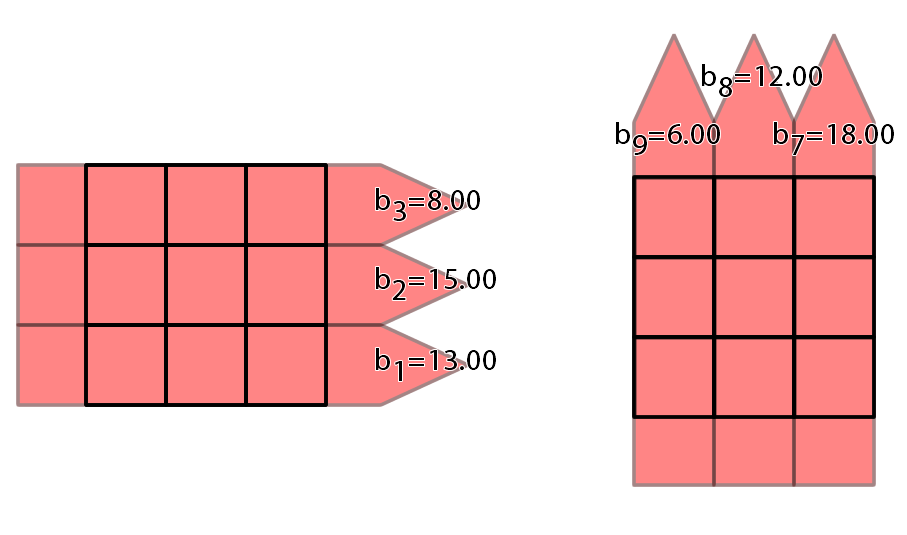
\includegraphics[width=11cm]{01_feixes_horizontais.fw.png}
    
    Feixes verticais e horizontais.
\end{center}

\begin{center}
    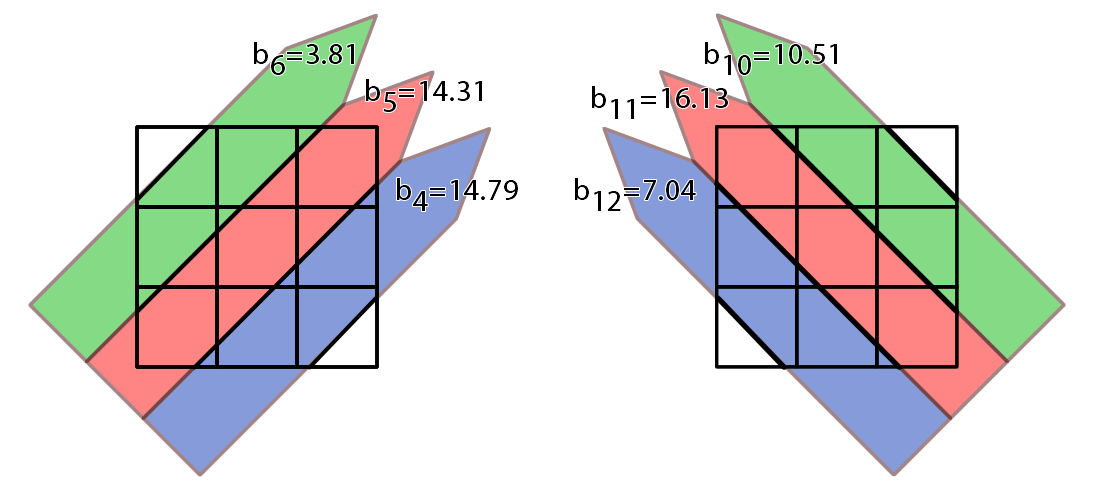
\includegraphics[width=11cm]{02_feixes_diagonais.fw.png}
    
    Feixes diagonais.
\end{center}

Neste caso portanto, independentemente do método escolhido teremos sempre 12 equações de feixe (pois temos 12 feixes).


\subsection{Usando o Método do Centro do Pixel}

Os coeficientes $a_{ij}$ no caso do método do centro do pixel são da seguinte forma:

$$a_{ij}=\begin{cases}
1&{,}\ se\ o\ i-esimo\ feixe\ passa\ pelo\ centro\ do\ j-esimo\ pixel\\
0&{,}\ caso\ contrario
\end{cases}$$

Para o caso em que os feixes são verticais e horizontais tem-se o seguinte esquema, destacando o centro dos pixels:

\begin{center}
    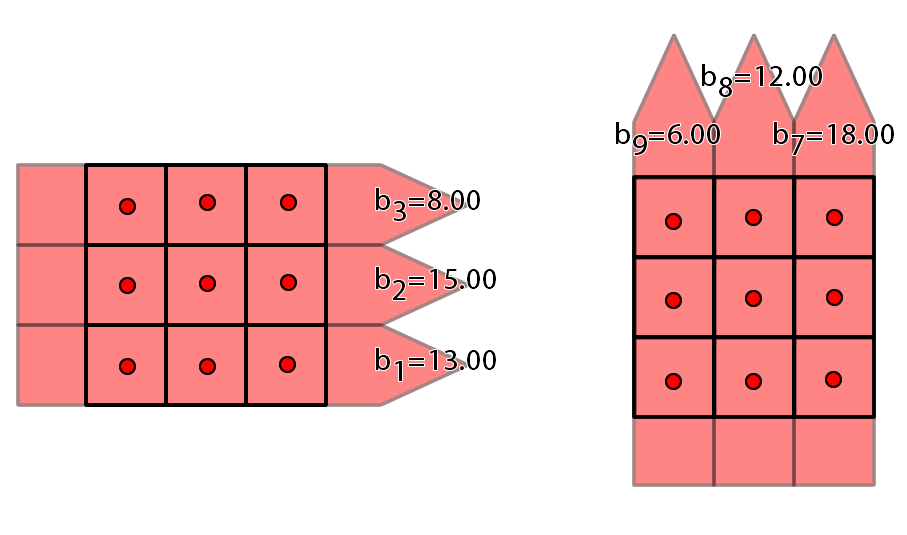
\includegraphics[width=11cm]{03_feixes_horizontais_centro_pixel.fw.png}
    
    Centros destacados: Feixes verticais e horizontais.
\end{center}

Como pode-se perceber, o feixe 3 passa pelo centro dos pixels 1, 2 e 3. Logo a equação de feixe correspondente será:

$$x_1+x_2+x_3=b_3$$

Analogamente para os outros 5 feixes, temos:

$$x_4+x_5+x_6=b_2$$
$$x_7+x_8+x_9=b_1$$
$$x_1+x_4+x_7=b_9$$
$$x_2+x_5+x_8=b_8$$
$$x_3+x_6+x_9=b_7$$\\

Já no caso dos feixes diagonais temos a seguinte situação:

\begin{center}
    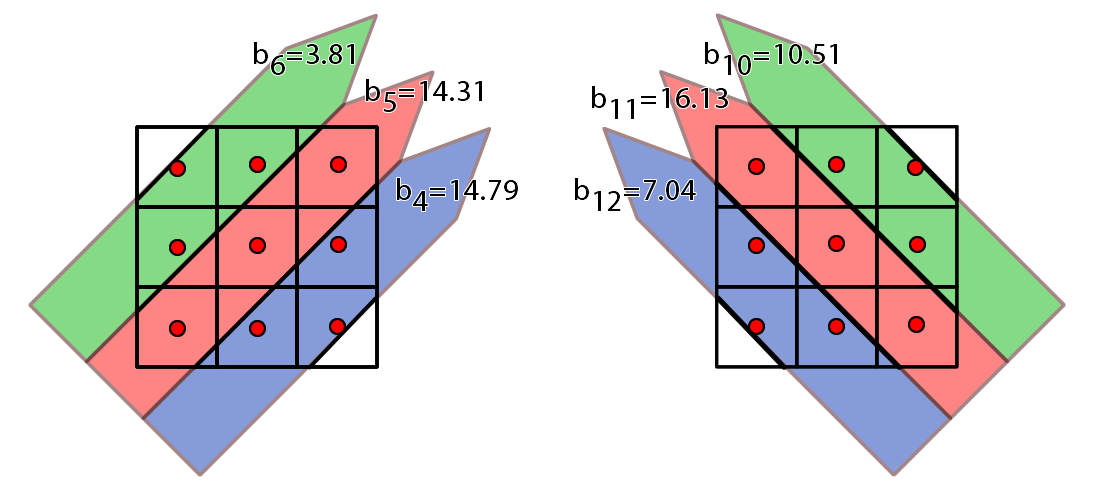
\includegraphics[width=11cm]{04_feixes_diagonais_centro_pixel.fw.png}
    
    Centros destacados: Feixes diagonais.
\end{center}

Nota-se que o feixe 6 passa pelo centro dos pixels 1, 2 e 4, logo a equação deste feixe é dada por:

$$x_1+x_2+x_4=b_6$$

Fazendo o mesmo procedimento para os outros 5 feixes diagonais temos:

$$x_3+x_5+x_7=b_5$$
$$x_6+x_8+x_9=b_4$$
$$x_2+x_3+x_6=b_{10}$$
$$x_1+x_5+x_9=b_{11}$$
$$x_4+x_7+x_8=b_{12}$$


\subsubsection{Equações: método do centro do pixel}

Juntando as equações acima e substituindo os valores de $b_1\  ...\  b_{12}$ pelos valores numéricos dados, temos que \textbf{as 12 equações de feixe para o caso do método do centro do pixel são}:

$$\boxed{\ \begin{matrix}
x_1+x_2+x_3=8.00\\
x_4+x_5+x_6=15.00\\
x_7+x_8+x_9=13.00\\
x_1+x_4+x_7=6.00\\
x_2+x_5+x_8=12.00\\
x_3+x_6+x_9=18.00\\
x_1+x_2+x_4=3.81\\
x_3+x_5+x_7=14.31\\
x_6+x_8+x_9=14.79\\
x_2+x_3+x_6=10.51\\
x_1+x_5+x_9=16.13\\
x_4+x_7+x_8=7.04
\end{matrix}\ }$$


\subsection{Usando o Método da Reta Central}

No método da reta central os coeficientes $a_{ij}$ são definidos como:

$$a_{ij}=\left(\frac{\begin{matrix}
\mathrm{comprimento\ da\ reta\ central\ do\ i-esimo\ feixe}\ \mathrm{que\ fica\ no\ j-esimo\ pixel}
\end{matrix}}{\mathrm{l\arg ura\ do\ j-esimo\ pixel}}\right)$$

Como estamos considerando que a largura de todos os pixels é igual a $L_{pixel}=x$, então os coeficientes $a_{ij}$ ficam:

$$a_{ij}=\left(\frac{\begin{matrix}
\mathrm{comprimento\ da\ reta\ central\ do\ i-esimo\ feixe}\ \mathrm{que\ fica\ no\ j-esimo\ pixel}
\end{matrix}}{x}\right)$$

Quando os feixes passam paralelamente aos lados temos que o comprimento da reta central que fica no interior de cada pixel é igual a própria largura do pixel, como pode ser visto na imagem abaixo:

\begin{center}
    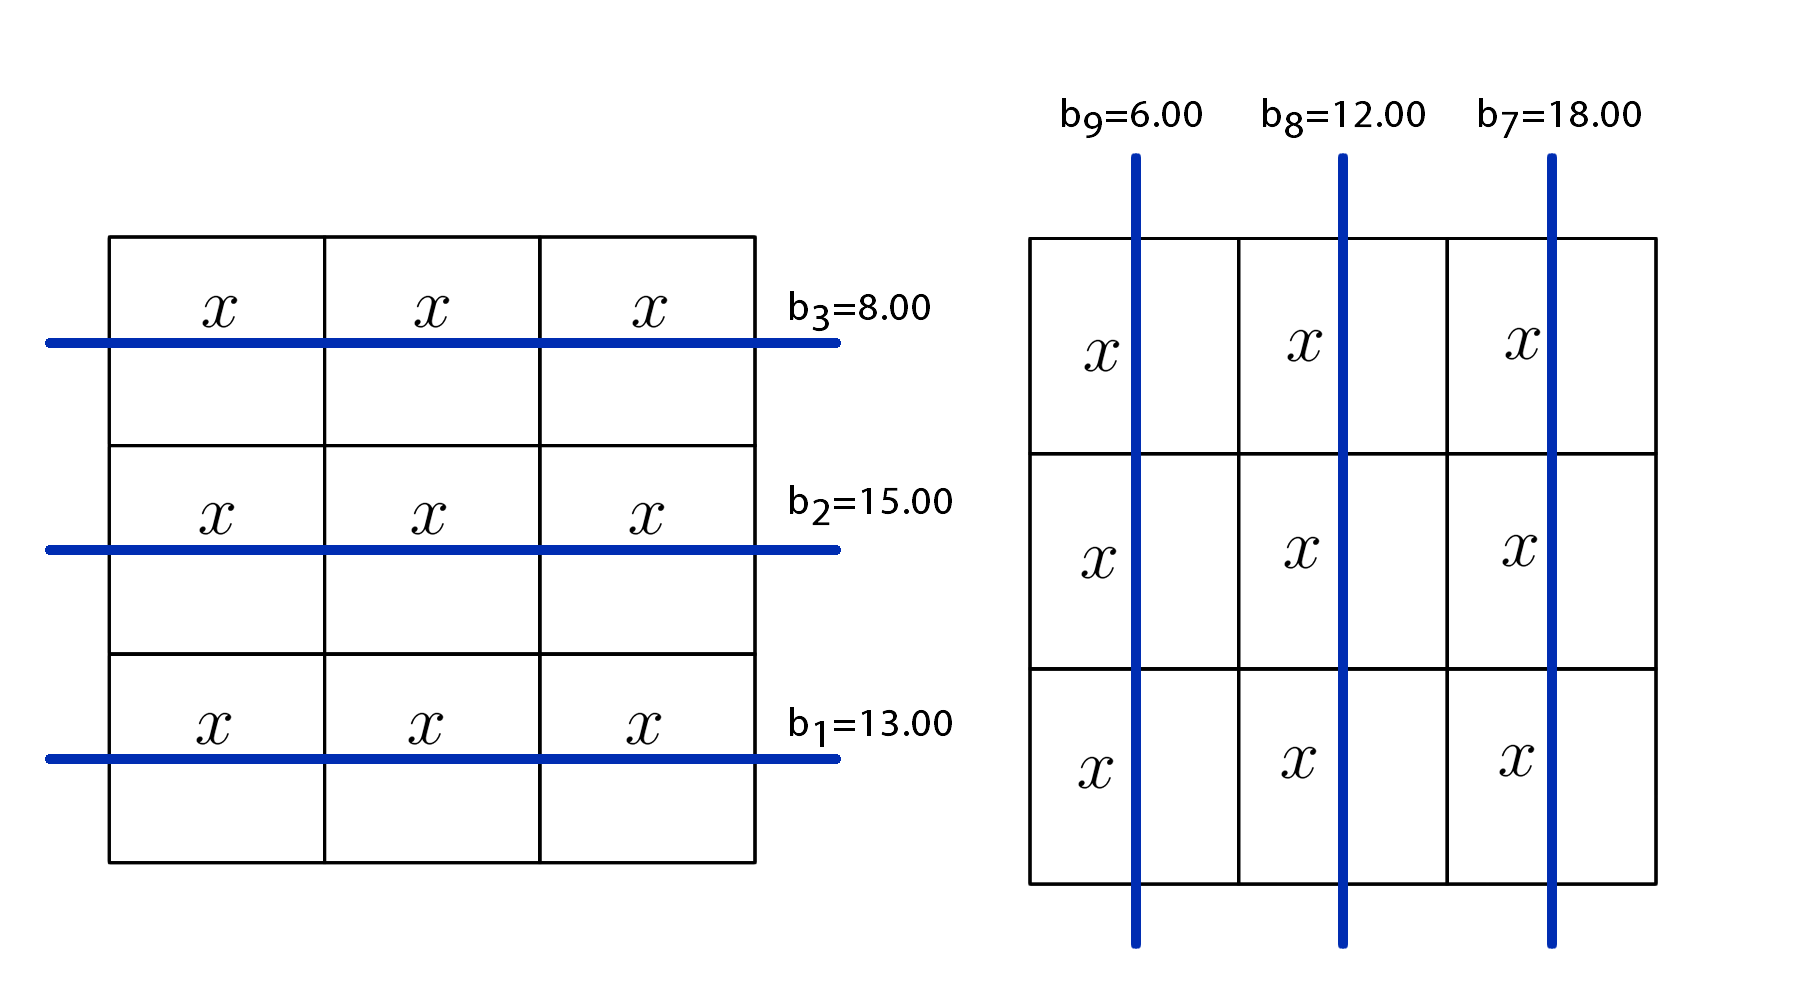
\includegraphics[width=13cm]{09_reta_central_vertical_horizontal.fw.png}
    
    Retas centrais: Feixes verticais e horizontais.
\end{center}

Portanto nos casos em que os feixes são $i=1, 2, 3, 7, 8, 9$, os valores de $a_{ij}$ são tais que:

$$a_{ij}=\begin{cases}
\frac{x}{x}=1&{,}\ se\ o\ i-esimo\ feixe\ atravessa\ o\ j-esimo\ pixel\\
&\\
\frac{0}{x}=0&{,}\ caso\ contrario
\end{cases}$$

Então para estes feixes temos as seguintes equações:

$$x_1+x_2+x_3=b_3$$
$$x_4+x_5+x_6=b_2$$
$$x_7+x_8+x_9=b_1$$
$$x_1+x_4+x_7=b_9$$
$$x_2+x_5+x_8=b_8$$
$$x_3+x_6+x_9=b_7$$\\

Já nos casos em que os feixes são diagonais, as retas centrais destes feixes são divididas pelas delimitações dos pixels nos segmentos de reta 1, 2 e 3. Como pode ser visto abaixo:

\begin{center}
    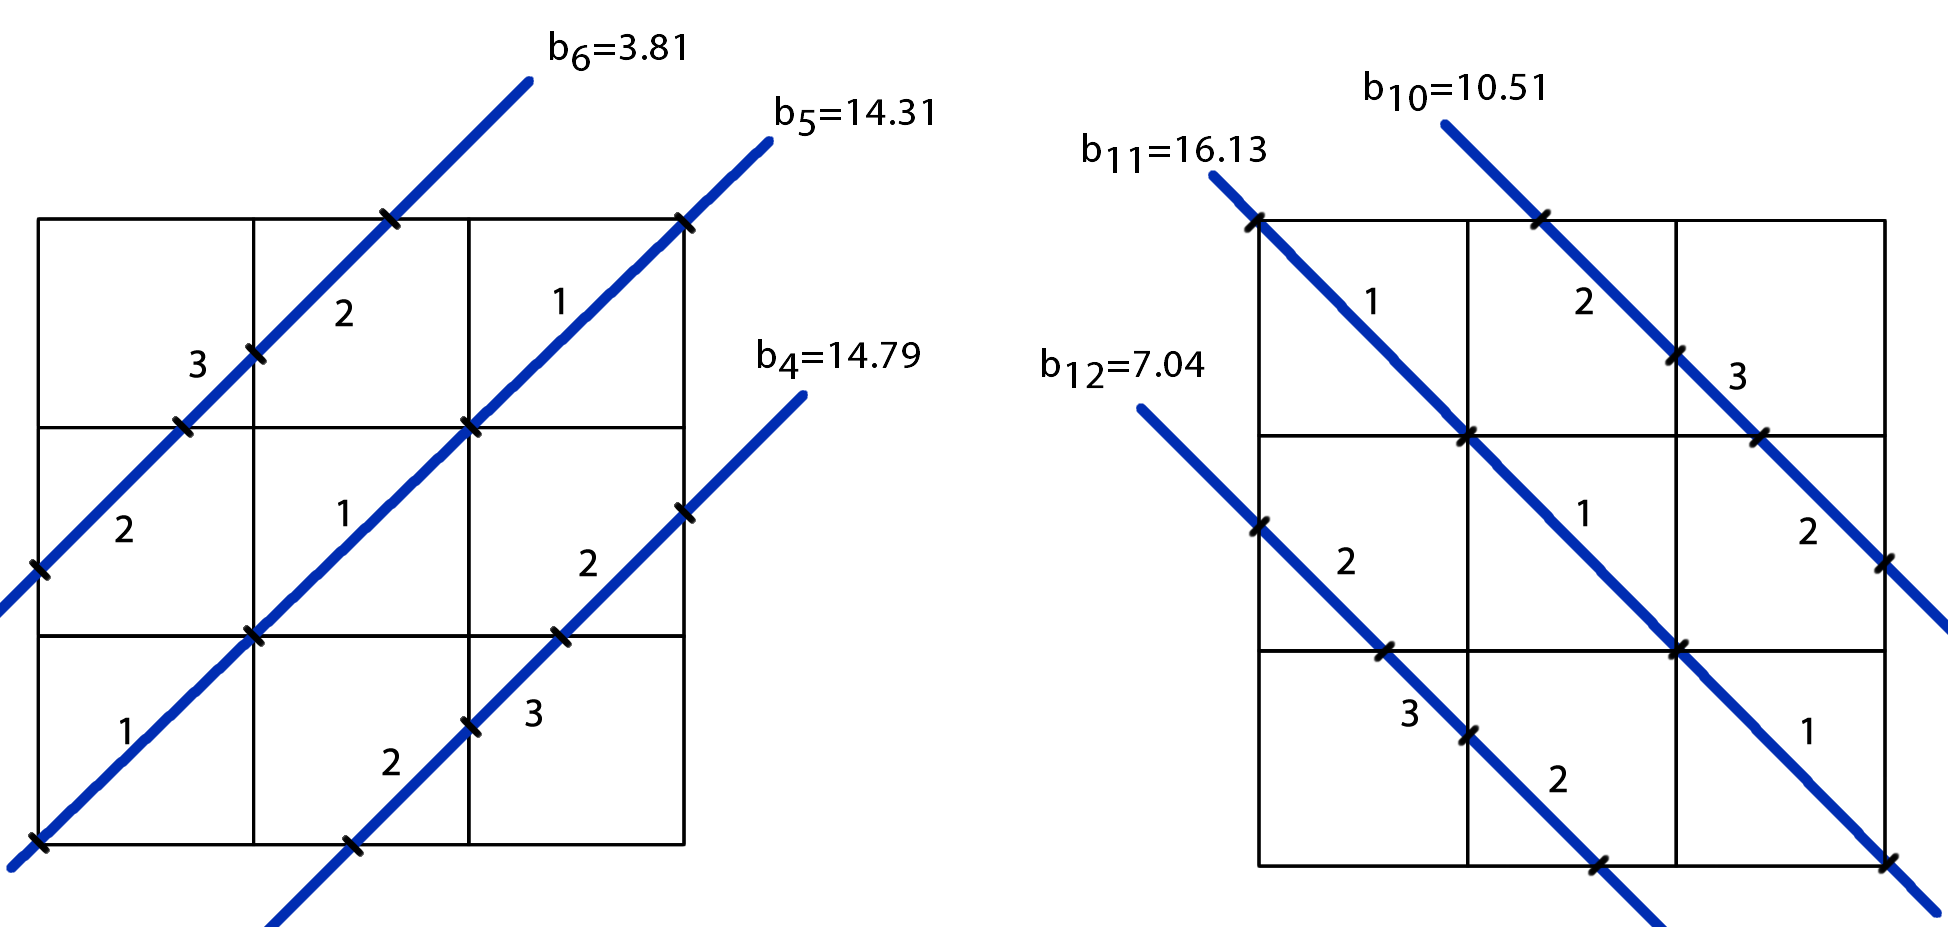
\includegraphics[width=13cm]{10_reta_central_diagonais.fw.png}
    
    Retas centrais: Feixes diagonais.
\end{center}

Sendo o comprimento desses segmentos de reta denotados por $L_1$, $L_2$ e $L_3$, temos que por geometria simples as suas medidas são dadas por:\\

\textbf{Comprimento de $L_1$}

$$L_1=x\sqrt{2}$$
$$\boxed{\ \ L_1=1.41421\cdot x\ \ }$$

\textbf{Comprimento de $L_2$}

$$L_2=x\left(2\sqrt{2}-2\right)$$
$$\boxed{\ \ L_2=0.82842\cdot x\ \ }$$

\textbf{Comprimento de $L_3$}

$$L_3=x\left(2-\sqrt{2}\right)$$
$$\boxed{\ \ L_3=0.58578\cdot x\ \ }$$\\

Com os valores de $L_1$, $L_2$ e $L_3$ calculados, analisaremos agora a trajetória de cada reta central para determinar as equações destes feixes diagonais.

A reta central do feixe 6 passa com comprimento $L_2$ pelo pixel 4, com comprimento $L_3$ pelo pixel 1, e com comprimento $L_2$ pelo pixel 2. Então a equação do feixe 6 será:

$$\frac{L_2}{x}x_4+\frac{L_3}{x}x_1+\frac{L_2}{x}x_2=b_6$$

Seguindo o mesmo raciocínio para os feixes 4, 5, 10, 11 e 12, temos as seguintes equações:

$$\frac{L_2}{x}x_8+\frac{L_3}{x}x_9+\frac{L_2}{x}x_6=b_4$$
$$\frac{L_1}{x}x_7+\frac{L_1}{x}x_5+\frac{L_1}{x}x_3=b_5$$
$$\frac{L_2}{x}x_2+\frac{L_3}{x}x_3+\frac{L_2}{x}x_6=b_{10}$$
$$\frac{L_1}{x}x_1+\frac{L_1}{x}x_5+\frac{L_1}{x}x_9=b_{11}$$
$$\frac{L_2}{x}x_4+\frac{L_3}{x}x_7+\frac{L_2}{x}x_8=b_{12}$$

\subsubsection{Equações: Método da Reta Central}
Substituindo os valores de $b_1\ ...\ b_12$ e de $L_1$, $L_2$ e $L_3$ nas 12 equações acima, temos que as equações no caso do método da reta central são:

$$\boxed{\ \ \begin{matrix}
x_1+x_2+x_3=8.00\\
x_4+x_5+x_6=15.00\\
x_7+x_8+x_9=13.00\\
x_1+x_4+x_7=6.00\\
x_2+x_5+x_8=12.00\\
x_3+x_6+x_9=18.00\\
0.82842\cdot x_4+0.58578\cdot x_1+0.82842\cdot x_2=3.81\\
1.41421\cdot x_7+1.41421\cdot x_5+1.41421\cdot x_3=14.31\\
0.82842\cdot x_8+0.58578\cdot x_9+0.82842\cdot x_6=14.79\\
0.82842\cdot x_2+0.58578\cdot x_3+0.82842\cdot x_6=10.51\\
1.41421\cdot x_1+1.41421\cdot x_5+1.41421\cdot x_9=16.13\\
0.82842\cdot x_4+0.58578\cdot x_7+0.82842\cdot x_8=7.04
\end{matrix}\ }$$

\subsection{Usando o Método da Área}

Por definição, os coeficientes $a_{ij}$ no método da área são dados por:

$$a_{ij}=\left(\frac{\mathrm{area\ do\ i-esimo\ feixe\ que\ fica\ no\ j-esimo\ pixel}}{\begin{matrix}
\mathrm{area\ do\ i-esimo\ feixe\ que\ ficaria\ no\ j-esimo\ pixel\ se\ o\ i-esimo}\\
\mathrm{feixe\ atravessasse\ o\ j-esimo\ pixel\ paralelamente\ aos\ lados}
\end{matrix}}\right)$$

Considerando a largura de cada pixel como $x$, então a área de cada um dos pixels é:

$$A_{pixel}=x^2$$

Então neste caso os coeficientes $a_{ij}$ são:

$$a_{ij}=\left(\frac{\mathrm{area\ do\ i-esimo\ feixe\ que\ fica\ no\ j-esimo\ pixel}}{x^2}\right)$$

Nos casos em que os feixes atravessam paralelamente aos lados, isto é nos casos de feixe vertical e horizontal, pelo fato de a largura do feixes ser a mesma largura dos pixels, então os feixes ocupam totalmente a área dos pixels que atravessam. Então os valores de $a_{ij}$ nos casos em que $i=1, 2, 3, 7, 8, 9$, são dados por:

$$a_{ij}=\begin{cases}
\frac{x^2}{x^2}=1&{,}\ se\ o\ i-esimo\ feixe\ atravessa\ o\ j-esimo\ pixel\\
&\\
\frac{0}{x^2}=0&{,}\ caso\ contrario
\end{cases}$$\\

Assim, como nos outros casos, as equações de feixe em que $i=1, 2, 3, 7, 8, 9$ são:

$$x_1+x_2+x_3=b_3$$
$$x_4+x_5+x_6=b_2$$
$$x_7+x_8+x_9=b_1$$
$$x_1+x_4+x_7=b_9$$
$$x_2+x_5+x_8=b_8$$
$$x_3+x_6+x_9=b_7$$

Já no caso dos feixes diagonais, são formadas áreas com medidas de 5 tamanhos diferentes, como indicado nas numerações de 1 a 5 abaixo:

\begin{center}
    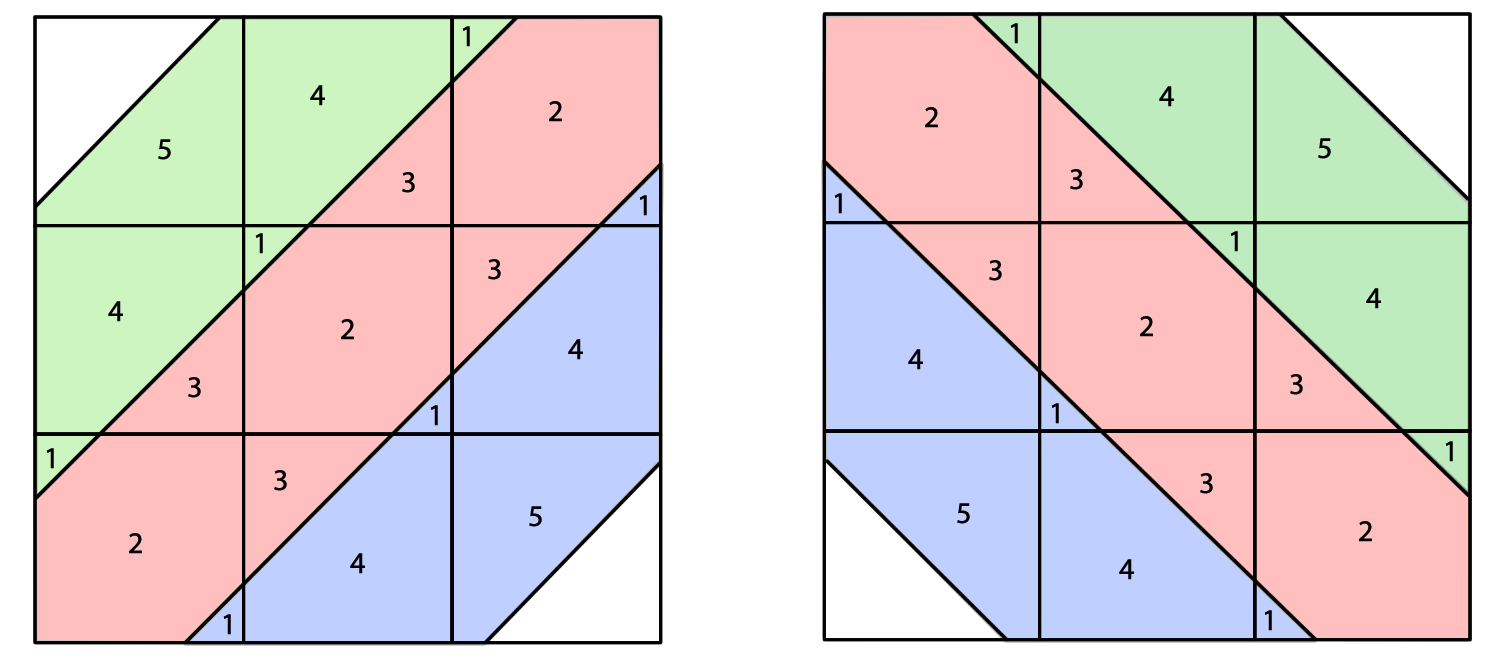
\includegraphics[width=11cm]{05_areas_diagonais.fw.png}
    
    Feixes diagonais: áreas de 5 tamanhos diferentes.
\end{center}

Precisamos agora calcular as áreas $A_1$, $A_2$, $A_3$, $A_4$ e $A_5$ associadas respectivamente a cada uma das numerações 1, 2, 3, 4 e 5 na imagem acima.\\

\textbf{Calculando área $A_1$}\\

Sendo a largura dos pixels igual a $x$, então temos o seguinte esquema para as medias da base e altura para qualquer um dos triângulos identificados com o número 1:

\begin{center}
    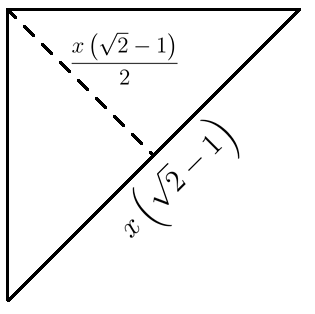
\includegraphics[width=6cm]{06_area_1.fw.png}
    
    Área 1: Base e altuda dos triangulos 1.
\end{center}

Portanto a área $A_1$ é:

$$A_1=\frac{base\cdot altura}{2}$$
$$A_1=\frac{x\left(\sqrt{2}-1\right)\cdot \frac{x\left(\sqrt{2}-1\right)}{2}}{2}$$
$$A_1=\frac{x^2\left(\sqrt{2}-1\right)^2}{4}$$
$$A_1=x^2\cdot \frac{3-2\sqrt{2}}{4}$$
$$\boxed{\ \ A_1=0.04289\cdot x^2\ }$$

\textbf{Calculando área $A_2$}\\

A área $A_2$ é obtida subtraindo a área de um pixel ($x^2$) por 2 vezes a área $A_1$, temos então:

$$A_2=x^2-2\cdot A_1$$
$$A_2=x^2-2\cdot \left(x^2\cdot \frac{3-2\sqrt{2}}{4}\right)$$
$$A_2=x^2\cdot \left(1-\frac{3-2\sqrt{2}}{2}\right)$$
$$\boxed{\ \ A_2=0.91421\cdot x^2\ \ }$$

\textbf{Calculando área $A_3$}\\

O triângulo da área 3 tem como base e altura as seguintes medidas:

\begin{center}
    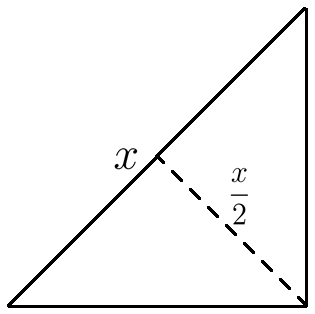
\includegraphics[width=6cm]{07_area_3.fw.png}
    
    Área 3: Base e altuda dos triangulos 3.
\end{center}

Assim, a área $A_3$ é dada por:

$$A_3=\frac{base\cdot altura}{2}$$
$$A_3=\frac{x\cdot \frac{x}{2}}{2}$$
$$A_3=\frac{x^2}{4}$$
$$\boxed{\ \ A_3=0.25\cdot x^2\ \ }$$

\textbf{Calculando área $A_4$}\\

A área 4 é obtida subtraindo-se a área de um pixel ($x^2$) pela área $A_3$. Então temos:

$$A_4=x^2-A_3$$
$$A_4=x^2-0.25\cdot x^2$$
$$\boxed{\ \ A_4=0.75\cdot x^2\ \ }$$

\textbf{Calculando área $A_5$}\\

A área 5 está destacada em azul na imagem abaixo e pode ser obtida subtraindo-se a área do pixel ($x^2$) pela área do triangulo em branco:

\begin{center}
    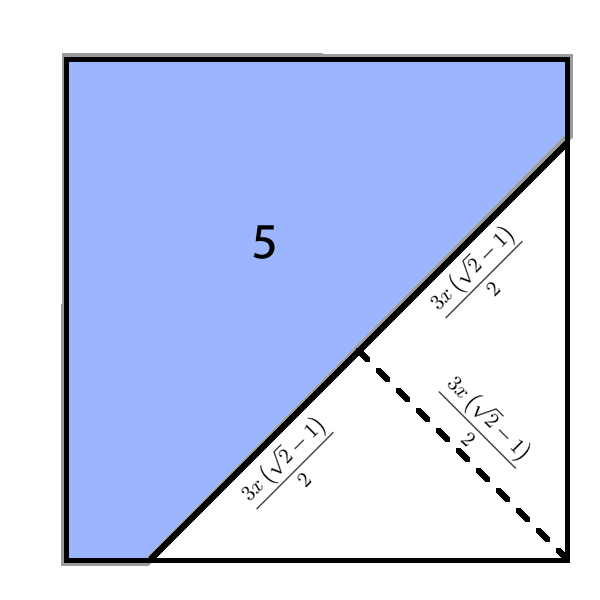
\includegraphics[width=8cm]{08_area_5.fw.png}
    
    Área 5: Área do pixel menos a área do triangulo branco.
\end{center}

Então a área $A_5$ é dada por:

$$A_5=x^2-\frac{base\cdot altura}{2}$$
$$A_5=x^2-\frac{3x\left(\sqrt{2}-1\right)\cdot \frac{3x\left(\sqrt{2}-1\right)}{2}}{2}$$
$$A_5=x^2-\frac{9x^2\left(\sqrt{2}-1\right)^2}{4}$$
$$A_5=\frac{4x^2-9x^2\left(3-2\sqrt{2}\right)}{4}$$
$$A_5=x^2\left[\frac{4-9\left(3-2\sqrt{2}\right)}{4}\right]$$
$$A_5=x^2\left[\frac{18\sqrt{2}-23}{4}\right]$$
$$\boxed{\ \ A_5=0.61396\cdot x^2\ \ }$$\\

Com as 5 áreas calculadas agora podemos encontrar as equações de feixe de todos os 6 feixes que passam na diagonal.

O feixe 6 passa pelos pixels 3, 5 e 7 cobrindo a área $A_1$. Passa pelos pixels 2 e 4 cobrindo a área $A_4$. E passa pelo pixel 1 cobrindo a área $A_5$. Então para o feixe 6 a equação será:

$$\frac{A_1}{x^2}\cdot \left(x_3+x_5+x_7\right)+\frac{A_4}{x^2}\cdot \left(x_2+x_4\right)+\frac{A_5}{x^2}\cdot x_1=b_6$$

O feixe 5 passa pelos pixels 3, 5 e 7 cobrindo a área $A_2$. E passa pelos pixels 2, 4, 6 e 8 cobrindo a área $A_3$. Logo equação do feixe 5 é: 

$$\frac{A_2}{x^2}\cdot \left(x_3+x_5+x_7\right)+\frac{A_3}{x^2}\cdot \left(x_2+x_4+x_6+x_8\right)=b_5$$

O feixe 4 passa pelos pixels 3, 5 e 7 cobrindo a área $A_1$. Passa pelos pixels 6 e 8 cobrindo a área $A_4$. E Passa pelo pixel 9 cobrindo a área $A_5$. Então a equação do feixe 4 é:

$$\frac{A_1}{x^2}\cdot \left(x_3+x_5+x_7\right)+\frac{A_4}{x^2}\cdot \left(x_6+x_8\right)+\frac{A_5}{x^2}\cdot x_9=b_4$$

O feixe 10 passa pelos pixels 1, 5 e 9 cobrindo a área $A_1$. Passa pelos pixels 2 e 6 cobrindo a área $A_4$. E passa pelo pixel 3 cobrindo a área $A_5$. Assim, temos que a equação do feixe 10 é:

$$\frac{A_1}{x^2}\cdot \left(x_1+x_5+x_9\right)+\frac{A_4}{x^2}\cdot \left(x_2+x_6\right)+\frac{A_5}{x^2}\cdot x_3=b_{10}$$

O feixe 11 passa pelos pixels 1, 5 e 9 cobrindo a área $A_2$. E passa pelos pixels 2, 4, 6 e 8 cobrindo a área $A_3$. Então neste caso temos:

$$\frac{A_2}{x^2}\cdot \left(x_1+x_5+x_9\right)+\frac{A_3}{x^2}\cdot \left(x_2+x_4+x_6+x_8\right)=b_{11}$$

E por último, o feixe 12 passa pelos pixels 1, 5 e 9 cobrindo a área $A_1$. Passa pelos pixels 4 e 8 cobrindo a área $A_4$. E passa pelo pixel 7 cobrindo a área $A_5$. Temos que a equação do feixe 12 é então:

$$\frac{A_1}{x^2}\cdot \left(x_1+x_5+x_9\right)+\frac{A_4}{x^2}\cdot \left(x_4+x_8\right)+\frac{A_5}{x^2}\cdot x_7=b_{12}$$

\subsubsection{Equações: método da área}
Juntando as 12 equações acima e substituindo os valores de $A_1\ ...\ A_5$ e de $b_1\ ...\ b_{12}$ temos:

$$\boxed{\ \ \begin{matrix}
x_1+x_2+x_3=8.00\\
x_4+x_5+x_6=15.00\\
\ x_7+x_8+x_9=13.00\\
x_1+x_4+x_7=6.00\\
\ x_2+x_5+x_8=12.00\\
x_3+x_6+x_9=18.00\\
0.04289\cdot \left(x_3+x_5+x_7\right)+0.75\cdot \left(x_2+x_4\right)+0.61396\cdot x_1=3.81\\
0.91421\cdot \left(x_3+x_5+x_7\right)+0.25\cdot \left(x_2+x_4+x_6+x_8\right)=14.31\\
0.04289\cdot \left(x_3+x_5+x_7\right)+0.75\cdot \left(x_6+x_8\right)+0.61396\cdot x_9=14.79\\
0.04289\cdot \left(x_1+x_5+x_9\right)+0.75\cdot \left(x_2+x_6\right)+0.61396\cdot x_3=10.51\\
0.91421\cdot \left(x_1+x_5+x_9\right)+0.25\cdot \left(x_2+x_4+x_6+x_8\right)=16.13\\
0.04289\cdot \left(x_1+x_5+x_9\right)+0.75\cdot \left(x_4+x_8\right)+0.61396\cdot x_7=7.04
\end{matrix}\ }$$

\section{Aplicação do Algoritmo generalizado}

Agora aplicaremos o algoritmo generalizado ( função \textit{Algoritmo 2} criada em \textit{Python} no inicio deste texto) para cada um dos três métodos vistos acima.

Para a reconstrução da imagem a partir do resultado do algorítimo generalizado primeiramente precisamos rearranjar os resultados para uma matriz quadrada, no exemplo da primeira saída do Algorítimo 2, por exemplo, a saída é um array com o resultado dos 9 pixels, porém precisamos colocá-los em uma matriz 3x3.

\begin{lstlisting}[language=Python, caption=Matriz Resultado, label=MatrizResultado]
#Cria a matriz com os resultados, a partir da tabela
def MatrizResultado(tab_df):
  
  tab_df = pd.DataFrame(tab_df) #Para Funcionar com df ou array
  resultado = tab_df.tail(1)
  len_tab = len(resultado.iloc[0])
  n = int(math.sqrt(len_tab))
  saida = np.zeros((n,n))

  #Resultados em Matriz Quadrada n por n
  for i in range (n):
    for j in range (n):
      saida[i][j] = resultado.iloc[0][i*n + j]

  return saida
\end{lstlisting}

Tendo o resultado podemos converter em imagem, usando as bibliotecas scikit-image e matplotlib, onde o pixel com maior valor ficará branco, o de menor valor preto, com os intermediários em tons de cinza.

\subsection{Caso do Método do Centro Pixel}

No código abaixo definimos as váriaveis com os valores encontrados na seção anterior.\\

\begin{lstlisting}[language=Python, caption=Definindo variáveis: Método do Centro do Pixel, label=Definindo variáveis: Método do Centro do Pixel]
#Matriz vetor a para o método do centro do pixel
a =np.matrix([[0,0,0,0,0,0,1,1,1],
              [0,0,0,1,1,1,0,0,0],
              [1,1,1,0,0,0,0,0,0],
              [0,0,0,0,0,1,0,1,1],
              [0,0,1,0,1,0,1,0,0],
              [1,1,0,1,0,0,0,0,0],
              [0,0,1,0,0,1,0,0,1],
              [0,1,0,0,1,0,0,1,0],
              [1,0,0,1,0,0,1,0,0],
              [0,1,1,0,0,1,0,0,0],
              [1,0,0,0,1,0,0,0,1],
              [0,0,0,1,0,0,1,1,0]])
#Valores de b
b = [13.0, 15.0, 8.0, 14.79, 14.31, 3.81, 18.0, 12.0, 6.0, 10.51, 16.13, 7.04]
xstar = np.zeros(9)   
\end{lstlisting}

Agora usamos o algoritmo generalizao para calcular qual será a imagem obtida, gerando a \textit{Tabela2}:\\

\begin{lstlisting}[language=Python, caption=Método do centro do Pixel: Construindo a imagem, label=Método do centro do Pixel: Construindo a imagem]
tab2 = Algoritmo2(a,b,xstar,45)

Tabela2 = pd.DataFrame()

#Df apartir de tab1 (resultado do ex1)
for i in range (len(tab2)):
  Tabela2 = Tabela2.append(tab2[i].tolist())

#Renomeando Colunas e resetando o index
Tabela2.rename({0:'x1', 1:'x2', 2:'x3', 
                3:'x4', 4:'x5', 5:'x6',
                6:'x7', 7:'x8', 8:'x9'}, inplace=True,axis=1)
Tabela2 = Tabela2.reset_index().drop('index',axis=1)
Tabela2.round(2)
\end{lstlisting}

O código acima gera a seguinte tabela como saída, lembrando que a última linha desta tabela representa a nossa resposta final, isto é, o valor da intensidade de coloração de nossa imagem como resposta.

\begin{center}

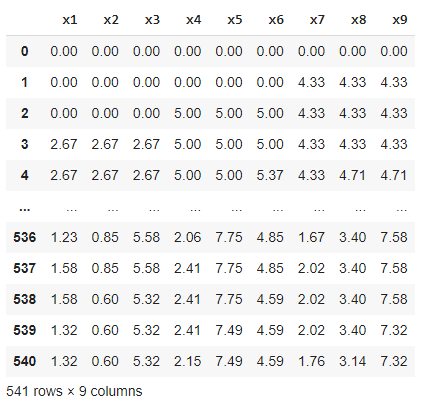
\includegraphics[width=11cm]{109_saida_tabela_2.PNG}

Tabela2: Última linha representa a imagem gerada pelo método do CENTRO DO PIXEL.   
    
\end{center}


\subsection{Caso do Método da Reta Central}

Fazendo o mesmo processo para os valores obtidos na seção 3 para o método da reta central temos:

\begin{lstlisting}[language=Python, caption=Método da reta central: construindo a imagem, label=Método da reta central: construindo a imagem]
#Matriz vetor a para o método da reta central
a_rc =np.matrix([[1,1,1,0,0,0,0,0,0],
                 [0,0,0,1,1,1,0,0,0],
                 [0,0,0,0,0,0,1,1,1],
                 [1,0,0,1,0,0,1,0,0],
                 [0,1,0,0,1,0,0,1,0],
                 [0,0,1,0,0,1,0,0,1],
                 [0.58578,0.82842,0,0.82842,0,0,0,0,0],
                 [0,0,1.41421,0,1.41421,0,1.41421,0,0],
                 [0,0,0,0,0,0.82842,0,0.82842,0.58578],
                 [0,0.82842,0.58578,0,0,0.82842,0,0,0],
                 [1.41421,0,0,0,1.41421,0,0,0,1.41421],
                 [0,0,0,0.82842,0,0,0.58578,0.82842,0]])
#Valores de b
b_rc = [8.0, 15.0, 13.0, 6.00, 12.00, 18.00, 3.81, 14.31, 14.79, 10.51, 16.13, 7.04]
xstar_rc = np.zeros(9)  

tab3 = Algoritmo2(a_rc,b_rc,xstar_rc,45)

Tabela3 = pd.DataFrame()

#Df apartir de tab1 (resultado do ex1)
for i in range (len(tab3)):
  Tabela3 = Tabela3.append(tab3[i].tolist())

#Renomeando Colunas e resetando o index
Tabela3.rename({0:'x1', 1:'x2', 2:'x3', 
                3:'x4', 4:'x5', 5:'x6',
                6:'x7', 7:'x8', 8:'x9'}, inplace=True,axis=1)
Tabela3 = Tabela3.reset_index().drop('index',axis=1)
Tabela3.round(2)
\end{lstlisting}

O código acima gera a seguinte \textit{Tabela3} em que a última linha representa a imagem contruída com o método da reta central.

\begin{center}
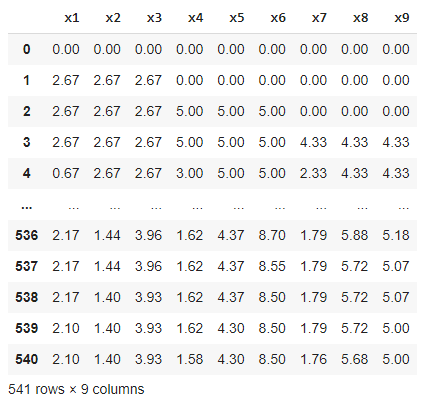
\includegraphics[width=11cm]{110_saida_tabela_3.PNG}

Tabela3: Última linha representa a imagem gerada pelo método da RETA CENTRAL.   
    
\end{center}

\subsection{Caso do Método da Área}

E mais uma vez, repetindo o processo anterior para os valores obtidos na seção 3 para o caso da Área, temos o seguinte processo que retorna os valores dos pixels da imagem gerada.

\begin{lstlisting}[language=Python, caption=Método da reta central: construindo a imagem, label=Método da reta central: construindo a imagem]
#Matriz vetor a para o método da Area
a_area =np.matrix([[1,1,1,0,0,0,0,0,0],
                 [0,0,0,1,1,1,0,0,0],
                 [0,0,0,0,0,0,1,1,1],
                 [1,0,0,1,0,0,1,0,0],
                 [0,1,0,0,1,0,0,1,0],
                 [0,0,1,0,0,1,0,0,1],
                 [0.61396,0.75,0.04289,0.75,0.04289,0,0.04289,0,0],
                 [0,0.25,0.91421,0.25,0.91421,0.25,0.91421,0.25,0],
                 [0,0,0.04289,0,0.04289,0.75,0.04289,0.75,0.61396],
                 [0.04289,0.75,0.61396,0,0.04289,0.75,0,0,0.04289],
                 [0.91421,0.25,0,0.25,0.91421,0.25,0,0.25,0.91421],
                 [0.04289,0,0,0.75,0.04289,0,0.61396,0.75,0.04289]])
#Valores de b
b_area = [8.0, 15.0, 13.0, 6.00, 12.00, 18.00, 3.81, 14.31, 14.79, 10.51, 16.13, 7.04]
xstar_area = np.zeros(9)

tab4 = Algoritmo2(a_area,b_area,xstar_area,45)

Tabela4 = pd.DataFrame()

#Df apartir de tab1 (resultado do ex1)
for i in range (len(tab4)):
  Tabela4 = Tabela4.append(tab4[i].tolist())

#Renomeando Colunas e resetando o index
Tabela4.rename({0:'x1', 1:'x2', 2:'x3', 
                3:'x4', 4:'x5', 5:'x6',
                6:'x7', 7:'x8', 8:'x9'}, inplace=True,axis=1)
Tabela4 = Tabela4.reset_index().drop('index',axis=1)
Tabela4.round(2)
\end{lstlisting}

\begin{center}
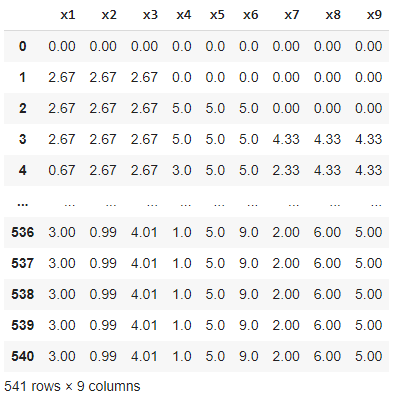
\includegraphics[width=11cm]{111_saida_tabela_4.PNG}

Tabela4: Última linha representa a imagem gerada pelo método da ÁREA.   

\end{center}

\subsection{Imagens Geradas}

A partir das variáveis \textit{Tabela2}, \textit{Tabela3} e \textit{Tabela4} geradas acima, iremos agora, usado a função \textit{Matriz Resultado} já definida e usando a biblioteca matplotlib, mostrar as imegens obtidas com os três métodos.

\begin{lstlisting}[language=Python, caption=Método da reta central: construindo a imagem, label=Método da reta central: construindo a imagem]
fig, (ax0, ax1, ax2) = plt.subplots(nrows=1, ncols=3, figsize=(16, 6),
                               sharex=True, sharey=True)

ax0.imshow(MatrizResultado(Tabela2), cmap=plt.cm.gray)
ax0.axis('off')
ax0.set_title('Centro do Pixel')
ax1.imshow(MatrizResultado(Tabela3), cmap=plt.cm.gray)
ax1.set_title('Reta Central')
ax1.axis('off')
ax2.imshow(MatrizResultado(Tabela4), cmap=plt.cm.gray)
ax2.set_title('Area')
ax2.axis('off')

plt.show()
\end{lstlisting}

\begin{center}
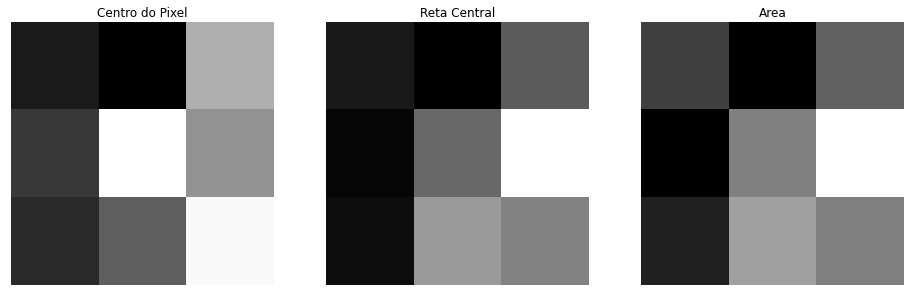
\includegraphics[width=16cm]{112_tres_metodos.PNG}

Tabela4: Comparação das imagens geradas pelos 3 métodos.   

\end{center}

\section{Desafio}

\subsection{Matriz a}

Tendo o modelo e os algorítimos para reconstrução da imagem, podemos testar para exemplo maiores e reais.

Inicialmente precisamos construir a matriz a para qualquer tamanho de imagem. Para facilitar a generalização das matrizes, escolhemos usar mais vetores nas diagonais, esses vetores passando pelas diagonais dos quadrados do pixels.

\begin{lstlisting}[language=Python, caption=Matriz a, label=Matriz a]
def cria_matriz_a_diagonal_1(n): # imagem n x n , com n*n pixels
    colunas = n*n
    linhas = (n-1)*2+1
    salto = n-1

    matriz = np.zeros((linhas, colunas))

    for i in range(int(linhas/2)+1):
        matriz[i][i] = 1
        for j in range(i):
            matriz[i][i+(j+1)*salto] = 1
  
    for i in range(int(linhas/2)+1, linhas):
        for j in range(colunas):
            matriz[i][j] = matriz[linhas-i-1][colunas-j-1]

    return matriz
  
def cria_matriz_a_diagonal_2(n): # imagem n x n , com n*n pixels
    colunas = n*n
    linhas = (n-1)*2+1
    salto = n+1

    matriz = np.zeros((linhas, colunas))

    for i in range(int(linhas/2)+1):
        matriz[i][n-1-i] = 1
        for j in range(i):
            matriz[i][n-1-i+(j+1)*salto] = 1
  
    for i in range(int(linhas/2)+1, linhas):
        for j in range(colunas):
            matriz[i][j] = matriz[linhas-i-1][colunas-j-1]

    return matriz
  
def cria_matriz_a_vertical(n): # imagem n x n , com n*n pixels
    linhas = n
    colunas = n*n
    salto = n

   matriz = np.zeros((linhas, colunas))

    for i in range(linhas):
      for j in range(linhas):
         matriz[i][i+salto*j] = 1
  
  return matriz
  
def cria_matriz_a_horizontal(n): # imagem n x n , com n*n pixels
    linhas = n
    colunas = n*n
    salto = n

    matriz = np.zeros((linhas, colunas))
    
    for i in range(linhas):
        for j in range(linhas):
          matriz[i][salto*i+j] = 1

    return matriz
  
def cria_matriz_a(n):
    md1 = cria_matriz_a_diagonal_1(n)
    md2 = cria_matriz_a_diagonal_2(n)
    mv = cria_matriz_a_vertical(n)
    mh = cria_matriz_a_horizontal(n)
    matriz_a = np.concatenate((md1,md2,mv,mh))
    return (np.asmatrix(matriz_a))
\end{lstlisting}

No nosso modelo a matriz 'a' terá número de colunas igual ao número de pixeis da imagem e número de linhas aproximadamente a 6 vezes o número de uma coluna/linha de pixeis. No modelo usado para 9 pixeis, a matriz 'a' tinha uma quantidade de linhas de 4 vezes o número de uma coluna/linha de pixel. Portanto o nosso modelo de criação da matriz a irá consumir mais memória, que funciona para imagens não muito grandes, mas para imagens maior que 512 x 512 pixel, teria que ter muita memória RAM disponível.

\subsection{Matriz b}

Com a matriz 'a' e a nossa imagem de teste. podemos construir uma lista com os resultados 'b'. Onde cada resultado representa a somatória do valor de cada pixel onde o feixe de raio x passa.

\begin{lstlisting}[language=Python, caption=Matriz b, label=Matriz b]
def CriaListab(matriz_a,imagem_np):
  len_img = len(imagem_np)
  pixel = len_img*len_img #n pixel para imagem quadrada
  vetor_pixel = [] #inicial
  for i in range (len_img):
    for j in range (len_img):
      vetor_pixel.append(imagem_np[i][j])
  vetor_pixel = np.array(vetor_pixel)

  b = []
  for k in range(len(matriz_a)):
    res = np.array(matriz_a[k])*vetor_pixel
    b.append(res.sum())

  return b
\end{lstlisting}

\subsection{Teste para uma imagem de 80 x 80 pixel}

\subsubsection{Imagem mais complexa}

Com o nosso modelo, podemos testar com imagens reais. Usaremos imagens da biblioteca scikit-image, inicialmente utilizaremos uma imagem mais complexa. Utilizaremos a imagem data.camera(), porém a imagem inicial possuí 512 x 512 pixel, então faremos o crop da imagem, pegando uma parte de 80 x 80 da imagem original

\begin{lstlisting}[language=Python, caption=Corte de imagem, label=camera80]
#Crop imagem camera em 80x80
camera = data.camera() #Imagem inicial

camera80 = np.zeros((80,80))
for i in range(80):
  for j in range(80):
    camera80[i][j]= camera[300+i][300+j] #parte central da imagem
\end{lstlisting}

\begin{lstlisting}[language=Python, caption=Teste 1 imagem 80 x 80, label=teste1_80]
matriz_a_teste = cria_matriz_a(80)
b_teste = CriaListab(matriz_a_teste,camera80)
x_teste = np.zeros(matriz_a_teste.shape[1])
teste80 = Algoritmo2(matriz_a_teste,b_teste,x_teste,50)
\end{lstlisting}

A saída na variável teste80 é a matriz coluna, com 6.400 valores, um para cada pixel da imagem resultante, a partir do vetor inicial zerado.


\begin{lstlisting}[language=Python, caption=Teste 1 imagem 80 x 80, label=teste1_80]
teste80_df = pd.DataFrame(teste80[-1]).T
teste80img = MatrizResultado(teste80_df)

#Criacao da imagem
fig, (ax0, ax1) = plt.subplots(nrows=1, ncols=2, figsize=(16, 6),
                               sharex=True, sharey=True)

ax0.imshow(camera80, cmap=plt.cm.gray)
ax0.axis('off')
ax0.set_title('Original')
ax1.imshow(teste80img, cmap=plt.cm.gray)
ax1.set_title('Gerada')
ax1.axis('off')

plt.savefig('camera80.png')
\end{lstlisting}

\begin{center}

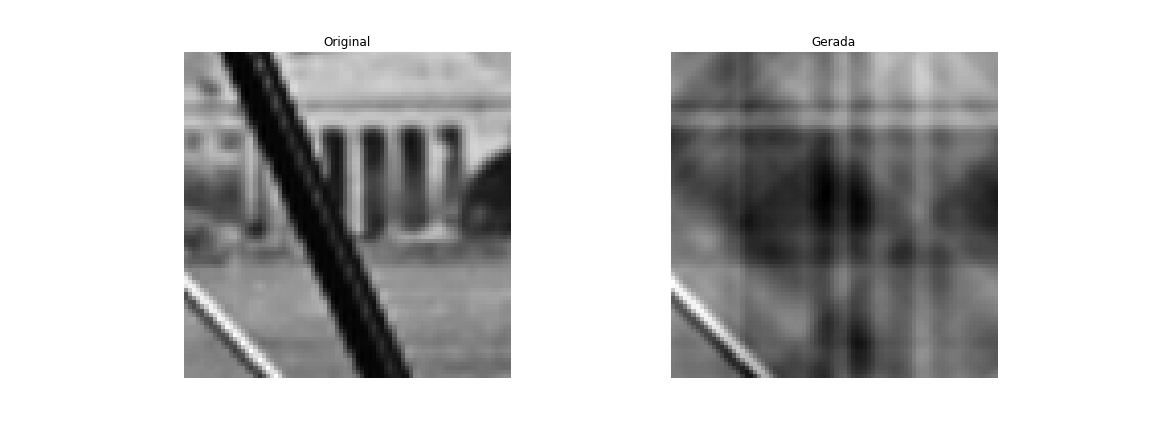
\includegraphics[width=16cm]{13_camera80.png}

Imagem original vs Imagem gerada pelo modelo   
    
\end{center}

Podemos observar que um pedaço da imagem que está exatamente a 45 graus foi reconstruída com boa precisão, mas o resto nem tanto. Isso se deve à limitação do nosso modelo que só reconstrói a imagem a partir de 4 feixes, em um caso real a máquina gira ao redor do paciente tendo vários ângulos, então o modelo com as limitações impostas não funciona muito bem com imagens mais complexas

\subsubsection{Imagem mais simples}

A imagem mais simples utilizada foi também retirada da biblioteca scikit-image, foram seguidos os mesmos passos anteriores, porém ao invés da imagem data.camera(), foi utilizada a imagem data.checkerboard() da biblioteca. A imagem escolhida é um tabuleiro de xadrez, onde só tem valor 255(branco) e 0 (preto), bem mais simples.

\begin{center}
    
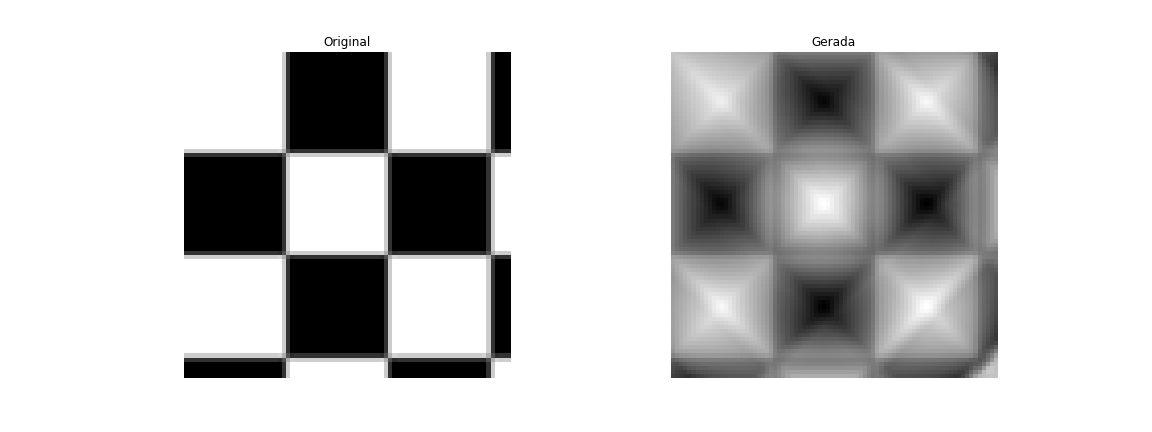
\includegraphics[width=16cm]{14_xadrez80_vetor0.png}

Imagem original vs Imagem gerada pelo modelo, Tabuleiro de xadrez partindo de um vetor zerado.  
    
\end{center}

\begin{center}
    
Podemos usar um vetor inicial diferente do zerado para avaliar o resultado.
Para isso foram seguidos os passos anteriores, só mudando a seguinte linha de código
\begin{lstlisting}
x_teste = np.random.randint(0,255,size=(matriz_a_teste.shape[1]))
\end{lstlisting}
criando assim um vetor inicial com valores aleatórios entre 0 e 255.

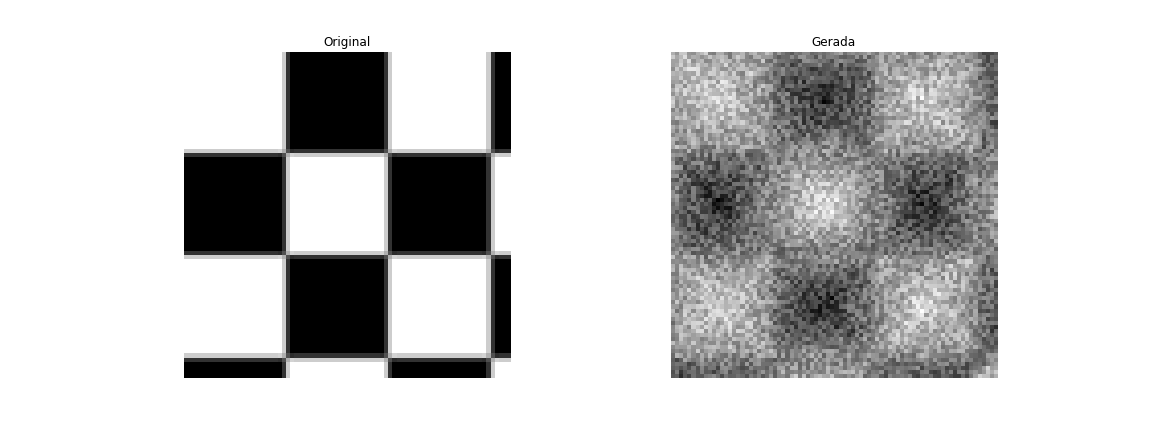
\includegraphics[width=16cm]{15_xadrez80_vetor_Aleatorio.png}

Imagem original vs Imagem gerada pelo modelo, Tabuleiro de xadrez partindo de um vetor aleatório inicial.   
    
\end{center}

No caso mais simples conseguimos ver mais claro a reconstrução das imagens pelo nosso modelo. Também foi possível ver a diferença quando partimos de vetores inicias diferentes.

\subsection{Teste para uma imagem de 512 x 512 pixel}

No caso para a reconstrução da imagem de 512 x 512 pixel, tivemos alguns problemas de memória RAM rodando o notebook com todas as funções. Então tivemos que fazer cada parte separada, e em um ambiente com mais memória RAM disponível.

O problema maior de memória foi para a criação da matriz a, pois no caso de 512 x 512, ela é uma matriz com 262144 colunas e 3070 linhas. E a grande maioria dos valores é zerado, então uma opção utilizada foi exportar em formato npz, que é um método no numpy onde podemos ter essa matriz com um arquivo bem menor, pois ela só guarda o valor e posição dos valores diferente de zero.
Ai tendo esse arquivo localmente, podemos gerar a matriz a, consumindo menos recurso de RAM, com o seguinte algorítimo

\begin{lstlisting}[language=Python, caption = reconstruindo a matriz a do arquivo npz]

matriz_a_512_csr = sparse.load_npz("../input/d/victorvianaom/matrizes-a/matriz_a_512_csr.npz")
matriz_512 = matriz_a_512_csr.todense()

\end{lstlisting}

\subsubsection{Imagem mais complexa}

Tendo a matriz 'a', podemos usar nossos algoritmos para reconstruir a figura data.camera(), cujo o tamanho original possui 512 x 512, a partir de um vetor zerado

\begin{lstlisting}[language=Python, caption = imagem 512 x 512]
camera = data.camera()
b_teste = CriaListab(matriz_512,camera)
x_teste = np.zeros(262144)
teste512 = Algoritmo2(matriz_512,b_teste,x_teste,20)

teste512_df = pd.DataFrame(teste512)
teste512img = MatrizResultado(teste512_df)

fig, (ax0, ax1) = plt.subplots(nrows=1, ncols=2, figsize=(16, 6),
                               sharex=True, sharey=True)

ax0.imshow(camera, cmap=plt.cm.gray)
ax0.axis('off')
ax0.set_title('Original')
ax1.imshow(teste512img, cmap=plt.cm.gray)
ax1.set_title('Gerada')
ax1.axis('off')

#plt.show()
plt.savefig("512_camera.png")
\end{lstlisting}

\begin{center}
    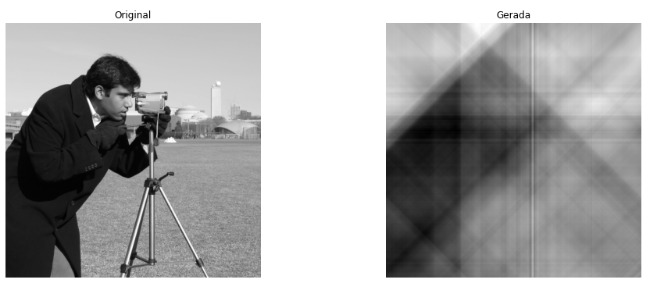
\includegraphics[width=16cm]{camera512.jpg}
    Figura mais complexa gerada pelo modelo
    
\end{center}

No caso da figura mais complexa, podemos ver só as partes mais escuras e mais claras, mas não da para definir muito bem qual era a imagem original, isso se deve ao fato do nosso modelo só pegar informações de 4 direções.

\subsubsection{Imagem mais simples}

Para a imagem mais simples, utilizamos a imagem do tabuleiro de xadrez (data.checkerboard()), porém a imagem original possui 200 x 200 pixel, então copiamos a imagem lado a lado algumas vezes, depois recortamos até ficar com 512 x 512, assim utilizando a mesma matriz 'a' anteriormente. Simulando com o algoritmo abaixo podemos ver o resultado com uma imagem mais simples.

\begin{lstlisting}[language=Python, caption = Imagem 512 x 512 mas simples]
b_teste = CriaListab(matriz_512,xadrez_512)
x_teste = np.zeros(262144)
teste512 = Algoritmo2(matriz_512,b_teste,x_teste,20)

teste512_df = pd.DataFrame(teste512)
teste512img = MatrizResultado(teste512_df)

fig, (ax0, ax1) = plt.subplots(nrows=1, ncols=2, figsize=(16, 6),
                               sharex=True, sharey=True)

ax0.imshow(xadrez_512, cmap=plt.cm.gray)
ax0.axis('off')
ax0.set_title('Original')
ax1.imshow(teste512img, cmap=plt.cm.gray)
ax1.set_title('Gerada')
ax1.axis('off')

#plt.show()
plt.savefig("512_xadrez.png")
\end{lstlisting}

\begin{center}

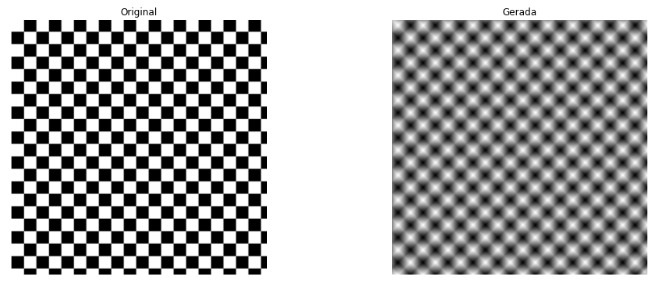
\includegraphics[width= 16cm]{saida512_2.jpg}

\end{center}

Na imagem mais simples da para ver o resultado bem mais consistente, vendo claramente que a imagem gerada partiu de um xadrez branco e preto

\bibliography{ref.bib}

\end{document}
